\documentclass[11pt,a4paper]{article}

% ------------------------------------------------------------------ packages
\usepackage[T1]{fontenc}
\usepackage[utf8]{inputenc}
\usepackage{lmodern}
\usepackage{microtype}
\usepackage[margin=2.4cm]{geometry}
\usepackage{graphicx}
\usepackage{booktabs}
\usepackage{tabularx}
\usepackage{array}
\usepackage{float}
\usepackage[font=small,labelfont=bf]{caption}
\usepackage{enumitem}
\usepackage[table]{xcolor}
\usepackage{amsmath}
\usepackage[round,authoryear]{natbib}
\usepackage{xurl}
\usepackage[colorlinks=true,linkcolor=blue!50!black,citecolor=blue!50!black,urlcolor=blue!50!black]{hyperref}
\usepackage{fancyhdr}
\usepackage{titlesec}
\usepackage[most]{tcolorbox}

\graphicspath{{../outputs/figures/}}
\setlength{\parskip}{0.45em}
\setlength{\parindent}{0pt}
\setlist{itemsep=0.15em, topsep=0.3em}
\renewcommand{\arraystretch}{1.15}
\titlespacing*{\section}{0pt}{1.1em}{0.5em}
\titlespacing*{\subsection}{0pt}{0.9em}{0.4em}
\titlespacing*{\subsubsection}{0pt}{0.8em}{0.3em}

\pagestyle{fancy}
\fancyhf{}
\fancyhead[L]{\small CS5805 Information Visualization -- Class Project}
\fancyhead[R]{\small Group [XX]}
\fancyfoot[C]{\small \thepage}
\renewcommand{\headrulewidth}{0.4pt}

\definecolor{acc}{HTML}{2a78d6}
\definecolor{okgreen}{HTML}{0c7a0c}
\definecolor{partly}{HTML}{b36b00}
\definecolor{nored}{HTML}{c0392b}
\newcommand{\accepted}{\textcolor{okgreen}{\textbf{Accepted}}}
\newcommand{\partly}{\textcolor{partly}{\textbf{Partly accepted}}}
\newcommand{\rejected}{\textcolor{nored}{\textbf{Rejected}}}

% Box for each hypothesis statement
\newtcolorbox{hyp}[1]{colback=acc!5, colframe=acc!70!black, boxrule=0.5pt,
  arc=1.5pt, left=5pt, right=5pt, top=3pt, bottom=3pt,
  fonttitle=\bfseries\small, title=#1}
% Box for the decision
\newtcolorbox{decision}{colback=black!3, colframe=black!40, boxrule=0.4pt,
  arc=1.5pt, left=5pt, right=5pt, top=3pt, bottom=3pt}

% Small marks-and-channels table
\newenvironment{mctable}{%
  \par\small\noindent
  \tabularx{\linewidth}{@{}>{\raggedright\arraybackslash}p{3.3cm}>{\raggedright\arraybackslash}p{3.0cm}X@{}}
  \toprule
  \textbf{Part of chart} & \textbf{Mark} & \textbf{Channel $\rightarrow$ data it shows}\\ \midrule}%
  {\bottomrule\endtabularx\par}

\newcommand{\rhoeq}[1]{$\rho = #1$}

\begin{document}

% ================================================================== title
\begin{titlepage}
\centering
\vspace*{1.5cm}
{\large [University name] \par}
{\large [Department / Programme] \par}
\vspace{0.4cm}
{\large CS5805 -- Information Visualization \par}
\vspace{2.2cm}
{\LARGE\bfseries Looking Inside Three Online Quizzes:\\[0.3em]
A Visual Study of Time, Difficulty and Re-attempts \par}
\vspace{0.8cm}
{\large Class Project Report \par}
\vspace{2.5cm}
{\large Group [XX] \par}
\vspace{0.5cm}
\begin{tabular}{ll}
\toprule
\textbf{Name} & \textbf{Index number} \\
\midrule
{[Member 1 name]} & {[Index number]} \\
{[Member 2 name]} & {[Index number]} \\
{[Member 3 name]} & {[Index number]} \\
{[Member 4 name]} & {[Index number]} \\
\bottomrule
\end{tabular}
\vfill
{\large November 2026 \par}
\end{titlepage}

% ================================================================== abstract
\begin{abstract}
\noindent
We studied 32,596 attempt records from three online quizzes taken by 6,656
students between March 2022 and March 2025. Each record has the start and end
time, the time taken, the total mark out of 10 and the mark for each of the
five questions. After cleaning the data, we used visualizations to check the
five hypotheses given in the brief and five hypotheses of our own. For each one
we picked a chart that suits the data type and the question, explained the
marks and channels we used, and backed the chart with a simple statistic.
Only one of the five given hypotheses was fully accepted: some questions are
clearly and consistently harder than others. More time goes with a slightly higher
score on a first attempt but not on re-attempts, there is a clear ``too fast'' zone
but not much of a ``too slow'' zone, and we found no sign that low performers
make more erratic progress. Our own hypotheses gave the most interesting
results. Students re-attempt mainly to reach 4 out of 10 and then stop. Before
May 2022 students could re-attempt straight away and those quick re-attempts
scored 9.2 out of 10 in about one minute, which points to answers being copied
from the feedback; after a two-hour wait was introduced this disappeared. We
also found that a student's Quiz 1 result says little about their later
quizzes, that later groups of students did better in Quiz 2, and that leaving a
question blank is a clear sign of low effort.
\end{abstract}

\tableofcontents
\newpage

% ================================================================== 1
\section{Introduction}

Online quizzes are now a normal part of most courses. Every time a student
opens a quiz, the learning management system (LMS) records when the attempt
started, when it ended and how many marks the student got for each question.
Teachers usually only look at the final mark, but these logs can tell us much
more: which questions are too hard, how students use their time, and how they
behave when they are allowed to try again.

In this project we were given the attempt logs of three quizzes from the same
course. A student could attempt each quiz many times. Our job had two parts.

\begin{itemize}
  \item \textbf{Task 1.} Check five given hypotheses (H1--H5) using suitable
        visualizations.
  \item \textbf{Task 2.} Come up with five more hypotheses (H6--H10) and check
        them in the same way.
\end{itemize}

For every hypothesis we say whether it can be accepted or rejected based on
the visualization, and we explain why we chose that chart in terms of
\emph{marks} and \emph{channels} \citep{munzner2014visualization}.

We tried to work the way a careful analyst would. Before drawing any chart we
spent time understanding the data, because several features of this dataset
(for example, attempts left open for days, and the very different behaviour on
first attempts and re-attempts) can easily lead to wrong conclusions if they
are ignored. Where a hypothesis could not be tested directly with the data we
have, we say so clearly and explain the indirect test we used instead.

The rest of the report is organised as follows. Section~\ref{sec:background}
gives background on quiz analytics and on the visualization principles we
followed. Section~\ref{sec:dataset} describes the dataset, the problems we
found in it and how we prepared it. Section~\ref{sec:method} explains our
method. Section~\ref{sec:results} presents the results for all ten hypotheses.
Section~\ref{sec:discussion} discusses what the results mean together, and
the limits of our study, and Section~\ref{sec:conclusion} concludes.

% ================================================================== 2
\section{Background}
\label{sec:background}

\subsection{Learning analytics and quiz logs}

Learning analytics is the use of data that learners leave behind to understand
and improve learning \citep{siemens2011penetrating}. Quiz logs are one of the
easiest sources because every LMS keeps them. Earlier work on large online
courses showed that students do not all behave the same way, and that grouping
them by their behaviour gives more useful insight than looking at averages
only \citep{kizilcec2013deconstructing}. We follow the same idea when we split
students into performance tiers and when we separate first attempts from
re-attempts.

Moodle, the LMS that produced this kind of export, describes how hard a
question is with the \emph{facility index}: the percentage of students who
got the question right \citep{moodle_stats}. A low facility index means a hard
question. We use the same measure in H2.

\subsection{Time on task and performance}

It is tempting to think that more time always means a better result, but
research shows that the link depends on the task and the person.
\citet{goldhammer2014time} studied more than a thousand adults in a large
computer-based test. In problem-solving tasks, spending more time was linked to
better results, and this effect was stronger for harder tasks and for less
skilled people. In routine reading tasks the effect was the opposite: skilled
people were fast \emph{and} correct. This is directly related to H1, H4 and H5.

Very short times can also be a sign of low effort. \citet{wise2005response}
showed that when students answer a question faster than it takes to read it,
they are usually guessing, and they called this ``rapid guessing''. We use this
idea when we look at very fast attempts (H5) and at questions left blank (H10).

\subsection{Re-attempts, feedback and ``gaming''}

Allowing several attempts can support learning, because taking a test is
itself a learning activity \citep{roediger2006test}. But re-attempts can also be
misused. \citet{baker2004offtask} described ``gaming the system'', where
students use the feedback or hints to get the right answer without thinking
about the content. In large online courses, \citet{alexandron2017copying}
found students who used extra accounts to collect correct answers and then
submitted them in their main account. Moodle gives teachers a simple tool
against fast repeated attempts: an \emph{enforced delay} between attempts
\citep{moodle_settings}. These ideas helped us explain H6 and H7.

People also often stop when a result is ``good enough'' instead of trying to
get the best result. \citet{simon1956rational} called this \emph{satisficing}.
H6 tests whether students re-attempt a quiz to pass or to get full marks.

Two statistical traps are relevant to this kind of data. First, if students
are grouped by a low first score, their next score will tend to be higher just
by chance; this is \emph{regression to the mean} \citep{barnett2005regression}.
Second, mixing two groups that behave differently (here, first attempts and
re-attempts) can hide or even reverse a trend that is present in each group;
this is known as Simpson's paradox \citep{simpson1951interpretation}.

\subsection{Visualization design principles}

We built every chart on a few well-known principles.

\begin{itemize}
  \item \textbf{Marks and channels.} A chart is made of \emph{marks} (points,
        lines, areas) and \emph{channels} that control how the marks look
        (position, length, colour, shape, size). The type of data decides which
        channels are suitable: ordered data should use ordered channels such as
        position or lightness, and categories should use identity channels such
        as colour hue or shape \citep{munzner2014visualization}.
  \item \textbf{Expressiveness and effectiveness.} A chart should show all the
        facts in the data and \emph{only} those facts, and the most important
        attribute should get the most accurate channel
        \citep{mackinlay1986automating}.
  \item \textbf{Ranking of channels.} People read position on a common scale
        most accurately, then length, then angle and area, and colour last
        \citep{cleveland1984graphical, heer2010crowdsourcing}. So we used
        position for the main comparison in every chart and avoided pie charts.
  \item \textbf{Data-ink and clutter.} Remove ink that does not carry data:
        light grid lines, no 3D, no heavy borders \citep{tufte2001visual}.
  \item \textbf{Show the distribution and the uncertainty.} Means alone can hide
        very different data \citep{weissgerber2015beyond}, so we show spreads
        (box plots, IQR bars) and 95\% confidence intervals.
  \item \textbf{Colour.} Use a sequential (one hue, light to dark) scale for
        ordered values, a diverging scale for values above and below a middle
        point, and distinct hues for categories, and make sure the colours are
        safe for colour-blind readers \citep{harrower2003colorbrewer}.
\end{itemize}

For changes of group membership over several steps we used an \emph{alluvial
diagram}, which was designed exactly to show how groups split and merge over
time \citep{rosvall2010mapping}.

% ================================================================== 3
\section{Dataset}
\label{sec:dataset}

\subsection{Source and attributes}

The data comes as three CSV files, one per quiz, exported from Moodle. Each row
is one attempt. Table~\ref{tab:dict} lists the columns.

\begin{table}[H]
\centering
\small
\caption{Columns in each quiz file.}
\label{tab:dict}
\begin{tabularx}{\linewidth}{@{}l l X@{}}
\toprule
\textbf{Column} & \textbf{Type} & \textbf{Description and notes} \\
\midrule
Student Code & Categorical (ID) & Anonymous student number, 0--6656. The same code is used in all three files, so students can be followed across quizzes. \\
State & Categorical & \texttt{Finished} or \texttt{In progress}. \\
Started on & Date-time & Start of the attempt, to the minute (e.g. \texttt{14 March 2022 6:55 AM}). \\
Completed & Date-time & End of the attempt, to the minute; ``-'' if not finished. \\
Time taken & Text $\rightarrow$ duration & e.g. \texttt{7 mins 25 secs}, \texttt{1 day 1 hour}, \texttt{1 year 362 days}. \\
Grade/10.00 & Ordered numeric & Total mark: 0, 2, 4, 6, 8 or 10. \\
Q. 1 \ldots{} Q. 5 /2.00 & Ordered numeric & Mark per question: 0 or 2 (no partial marks); ``-'' if no answer was given. \\
\bottomrule
\end{tabularx}
\end{table}

The quiz questions themselves are not included, so Question 1 of Quiz 1 and
Question 1 of Quiz 2 are different questions. In total there are 15 distinct
questions. In the rest of the report we write \textbf{Q1.4} to mean Quiz 1,
Question 4.

\subsection{What we found when we explored the data}

Before cleaning anything we profiled every column. The main findings were:

\begin{enumerate}
  \item \textbf{Size and time span.} 32,596 rows (Quiz 1: 13,989; Quiz 2:
        10,474; Quiz 3: 8,133) from 6,656 students, covering 14 March 2022 to
        22 March 2025. Almost every student (99.7\%) took the quizzes in order
        (1, then 2, then 3).
  \item \textbf{Unfinished attempts.} 189 rows are \texttt{In progress} and have
        no marks, no end time and no time taken. Student code 0 only appears in
        such rows.
  \item \textbf{Blank answers.} A ``-'' in a question column of a
        \emph{finished} attempt means the student did not answer it. We checked
        that the total grade always equals the sum of the question marks when
        ``-'' is counted as 0 (0 mismatches in 32,407 finished attempts).
        Blanks are rare except for two questions: Q1.4 and Q2.5 are left blank
        in about 9\% of first attempts, while every other question is under 1\%.
  \item \textbf{Very long times.} The quiz has no time limit. The median attempt
        takes about 6 minutes, but 4.4\% of finished attempts last more than an
        hour and some last for days, months or even almost two years. These are
        clearly tabs that were left open, not real working time
        (Figure~\ref{fig:overview}b).
  \item \textbf{Mixed time formats.} ``Time taken'' mixes seconds, minutes,
        hours, days and years, and long durations are rounded (``1 day 1
        hour''). Start and end times only have minute precision, so for short
        attempts the ``Time taken'' column is more precise than end minus start.
  \item \textbf{Many re-attempts.} 66\% of students re-attempted Quiz 1, 39\%
        re-attempted Quiz 2 and 18\% re-attempted Quiz 3. Some students made up
        to 7 attempts.
\end{enumerate}

\subsection{Preprocessing steps}

All steps are in \texttt{src/data\_prep.py} and are repeated every time the
code runs. Table~\ref{tab:clean} summarises them.

\begin{table}[H]
\centering
\small
\caption{Cleaning and preparation steps.}
\label{tab:clean}
\begin{tabularx}{\linewidth}{@{}c X r r@{}}
\toprule
\# & \textbf{Step and reason} & \textbf{Rows in} & \textbf{Rows out} \\
\midrule
1 & Load the three files and add a \texttt{quiz} column. & 32,596 & 32,596 \\
2 & Remove \texttt{In progress} attempts, because they have no marks. & 32,596 & 32,407 \\
3 & Parse dates; turn ``Time taken'' into seconds (handles years, days, hours, minutes, seconds). & 32,407 & 32,407 \\
4 & Turn ``-'' question marks into 0 and keep a separate \texttt{skipped} flag; check grade = sum of questions. & 32,407 & 32,407 \\
5 & Order each student's attempts on each quiz by start time; add attempt number, number of attempts, first/last flags, previous grade, change in grade and the waiting time since the previous attempt. & 32,407 & 32,407 \\
6 & Flag attempts longer than 60 minutes as \emph{long sessions} (1,436 attempts, 4.4\%). They stay in all score analyses but are left out of analyses that use time, unless we say otherwise. & 32,407 & 32,407 \\
7 & Add calendar fields (year, half-year, hour) and build a student table with first-attempt grades and a performance tier. & -- & 6,656 students \\
\bottomrule
\end{tabularx}
\end{table}

\textbf{Why 60 minutes?} Figure~\ref{fig:overview}b shows that time taken, on a
log scale, forms a clear hump between about 20 seconds and 40 minutes, and
then a long flat tail. A five-question quiz does not need an hour of active
work, so we treat anything longer as ``tab left open''. We did not delete these
rows, because their marks are still real; for H5 we even put them back on
purpose to see what happens to students who ``take too long''.

\textbf{Performance tiers.} Several hypotheses compare high and low performers.
We define a student's level by the \emph{average of their first-attempt grades
in the three quizzes}. First attempts are used because later attempts are
affected by what the student saw in the feedback. We then use simple, fixed
cut-offs: \textbf{Low} below 4 (2,174 students), \textbf{Medium} 4 to below 6
(2,978 students) and \textbf{High} 6 or more (1,504 students). For H3 we also
use a second definition as a check (see Section~\ref{sec:h3}).

\subsection{Overview of the data}

\begin{figure}[H]
\centering
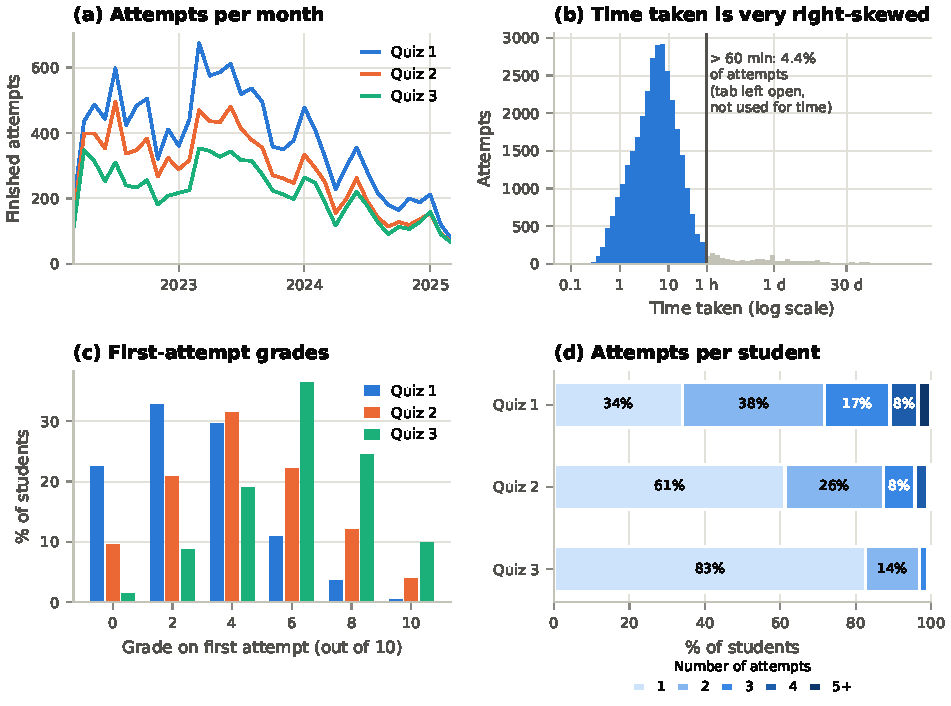
\includegraphics[width=\linewidth]{fig01_dataset_overview.pdf}
\caption{Dataset overview. (a) Number of finished attempts per month. (b)
Distribution of time taken on a log scale; grey bars are attempts longer than
60 minutes. (c) First-attempt grade distribution per quiz. (d) Share of
students by number of attempts.}
\label{fig:overview}
\end{figure}

Figure~\ref{fig:overview} gives a first picture. Activity was highest in 2023
and slowly fell after that (a). Quiz 1 is by far the hardest: 55\% of students
scored 0 or 2 on their first try, while Quiz 3 is the easiest with a mean
first-attempt grade of 6.1 (c). Because of this, Quiz 1 also has the most
re-attempts (d). These differences between the quizzes are large, so in most
charts we show the three quizzes separately rather than mixing them.

% ================================================================== 4
\section{Methodology}
\label{sec:method}

\subsection{Tools}

We used Python 3 with pandas for data handling \citep{mckinney2010pandas},
matplotlib for all charts \citep{hunter2007matplotlib} and SciPy for the
statistics \citep{virtanen2020scipy}. Everything runs from one command
(\texttt{python run\_all.py}) and takes about ten seconds. The script writes
every figure, the cleaned data and a \texttt{results.json} file with every
number we quote in this report, so the text and the charts always match.

\subsection{General approach}

For each hypothesis we followed the same five steps:
\begin{enumerate}
  \item Turn the hypothesis into something we can measure with the columns we
        have (and say so if we can only measure it indirectly).
  \item Choose the data subset carefully. The most important choice was to
        \textbf{separate first attempts from re-attempts}. A re-attempt is made
        after the student has seen the feedback, so its time and score mean
        something different. Mixing the two can reverse a trend (we show this
        in H1).
  \item Choose a chart based on the data types and the task, using the
        principles in Section~\ref{sec:background}.
  \item Add one or two simple statistics to support what the chart shows.
  \item Decide: \accepted, \partly{} or \rejected.
\end{enumerate}

\subsection{Statistical support}

The charts are our main evidence. The statistics only make sure we are not
fooled by noise. We used Spearman's rank correlation $\rho$ for relationships
(it works for skewed time data and ordered grades), chi-square tests with
Cram\'er's $V$ for comparing proportions, Mann--Whitney and Kruskal--Wallis
tests for comparing groups. We show 95\% confidence intervals everywhere: the
normal approximation for means and the bootstrap for medians
\citep{efron1993bootstrap}.

With more than 30,000 attempts almost every difference has $p < 0.001$, so a
small $p$-value alone does not mean a result matters. We therefore always look
at the \emph{size} of the effect. As a rough guide, we treat $|\rho| < 0.1$ as
negligible, 0.1--0.3 as weak and above 0.3 as moderate or strong.

\subsection{Design choices used in all figures}
\label{sec:design}

\begin{itemize}
  \item \textbf{Consistent colour meaning.} Quizzes always have the same hues
        (Quiz~1 blue, Quiz~2 orange, Quiz~3 green). These three colours were
        checked with a colour-vision-deficiency validator and stay apart for all
        common types of colour blindness. Student tiers always use one blue hue
        from light (Low) to dark (High), because tiers are \emph{ordered}.
        Up/same/down changes use a diverging red--grey--blue scale.
  \item \textbf{Position first.} The main comparison in every chart is on a
        common position scale. Colour is used for grouping, not for reading
        values.
  \item \textbf{Log scale for time.} Time taken is very right-skewed, so all
        time axes use a log scale with readable ticks (1, 2, 5, 10 minutes).
  \item \textbf{Uncertainty and spread.} Means are shown with 95\% confidence
        bands or bars; medians with inter-quartile ranges or bootstrap
        intervals; points with fewer than 30 attempts are hidden.
  \item \textbf{Direct labels and light chrome.} Where possible, lines are
        labelled at their ends instead of with a legend; grid lines are thin
        and light; no 3D, no pie charts, no dual axes (when we need counts next
        to a trend we use a second aligned panel instead of a second y-axis).
  \item \textbf{Small multiples.} When a chart would get crowded we split it
        into side-by-side panels with the same scales.
\end{itemize}

% ================================================================== 5
\section{Results}
\label{sec:results}

In this section we go through the ten hypotheses one by one. For each one we
state the hypothesis, explain how we turned it into something measurable, show
the chart, list its marks and channels, describe what we see and give a
decision.

% ---------------------------------------------------------------- Task 1
\subsection{Task 1: the given hypotheses}

% ............................................................ H1
\subsubsection{H1 -- Longer time, higher score?}
\label{sec:h1}

\begin{hyp}{H1}
Students who take longer to complete the quiz tend to score higher.
\end{hyp}

\textbf{How we tested it.} We compared time taken with the grade, separately
for first attempts and for re-attempts, and separately for each quiz. Attempts
over 60 minutes were left out because they do not show real working time.

\textbf{Why this chart.} The grade has only six possible values and there are
more than 30,000 attempts, so a normal scatter plot would be a few solid
stripes of overlapping dots and would hide the pattern. Instead, for each grade
we show the \emph{median} time and the middle 50\% of times (IQR). This keeps
both the trend and the spread visible. We put first attempts and re-attempts
in two panels with the same y-axis (small multiples), so the two can be
compared directly.

\begin{figure}[H]
\centering
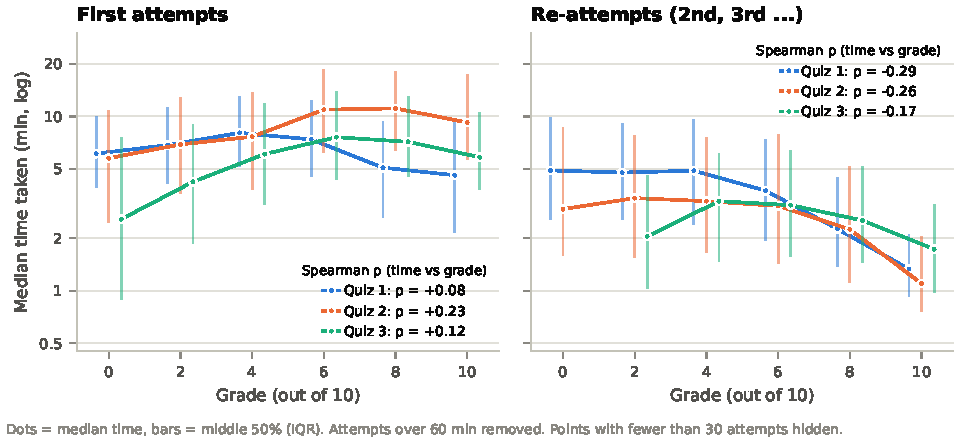
\includegraphics[width=\linewidth]{fig02_h1_time_vs_score.pdf}
\caption{H1. Median time taken (log scale) for each grade, with the
inter-quartile range. Left: first attempts. Right: re-attempts. Legends give
Spearman's $\rho$ between time and grade for each quiz.}
\label{fig:h1}
\end{figure}

\begin{mctable}
Median time per grade & Point & Vertical position (log) $\rightarrow$ median minutes; horizontal position $\rightarrow$ grade (ordered) \\
Spread & Line (vertical bar) & Length $\rightarrow$ inter-quartile range \\
Trend & Line connecting points & Slope $\rightarrow$ direction of change \\
Quiz & -- & Colour hue $\rightarrow$ quiz (categorical); small horizontal offset to avoid overlap \\
Attempt type & Separate panel & Spatial region $\rightarrow$ first vs.\ re-attempt \\
\end{mctable}

\textbf{What we see.} On \emph{first attempts} the lines go up from left to
right until about 6 or 8 marks: the median time rises from 6.0 minutes for a
grade of 0 to 8.5 minutes for a grade of 6. But the correlation is weak
(\rhoeq{0.08} for Quiz 1, 0.23 for Quiz 2 and 0.12 for Quiz 3), and students
with full marks were \emph{not} the slowest (6.5 minutes). On
\emph{re-attempts} the picture is reversed: the higher the grade, the shorter
the time, and a re-attempt with 10/10 took only about 1.3 minutes (\rhoeq{-0.17}
to $-0.29$). If we ignore the difference and put all attempts together, the
overall correlation becomes slightly negative (\rhoeq{-0.08}). This is a clear
case of Simpson's paradox: the two groups have opposite trends, and mixing them
hides both \citep{simpson1951interpretation}. The fast, high re-attempts are
explained in H7.

\begin{decision}
\textbf{Decision: \partly.} On a first attempt, taking longer goes with a
slightly higher score, but the link is weak ($\rho$ = 0.08--0.23) and it stops
at full marks. On re-attempts the opposite is true. So H1 is not true as a
general rule; it only holds weakly for first attempts.
\end{decision}

% ............................................................ H2
\subsubsection{H2 -- Are some questions consistently harder?}
\label{sec:h2}

\begin{hyp}{H2}
Some questions are consistently harder than others.
\end{hyp}

\textbf{How we tested it.} We measured difficulty with the facility index (\%
of first attempts that got the question right). ``Harder'' means a lower
facility index. ``Consistently'' needs a second check, so we tested whether the
same questions stay hard (i) for all three student tiers and (ii) across
the seven half-years in the data. We used first attempts only, because
re-attempts are affected by feedback.

\textbf{Why this chart.} Panel (a) is a heatmap because it gives a compact
overview of all 15 questions at once, with the exact value printed in each
cell, so readers do not have to judge colour alone. Panel (b) is a dot plot
because comparing tiers needs \emph{position on a common scale}, the most
accurate channel \citep{cleveland1984graphical}; the grey bar between the dots
shows the gap between Low and High students. Panel (c) is a second heatmap
with half-years as columns, so a stable ranking shows up as horizontal bands of
the same shade. Both heatmaps use the same sequential blue scale.

\begin{figure}[H]
\centering
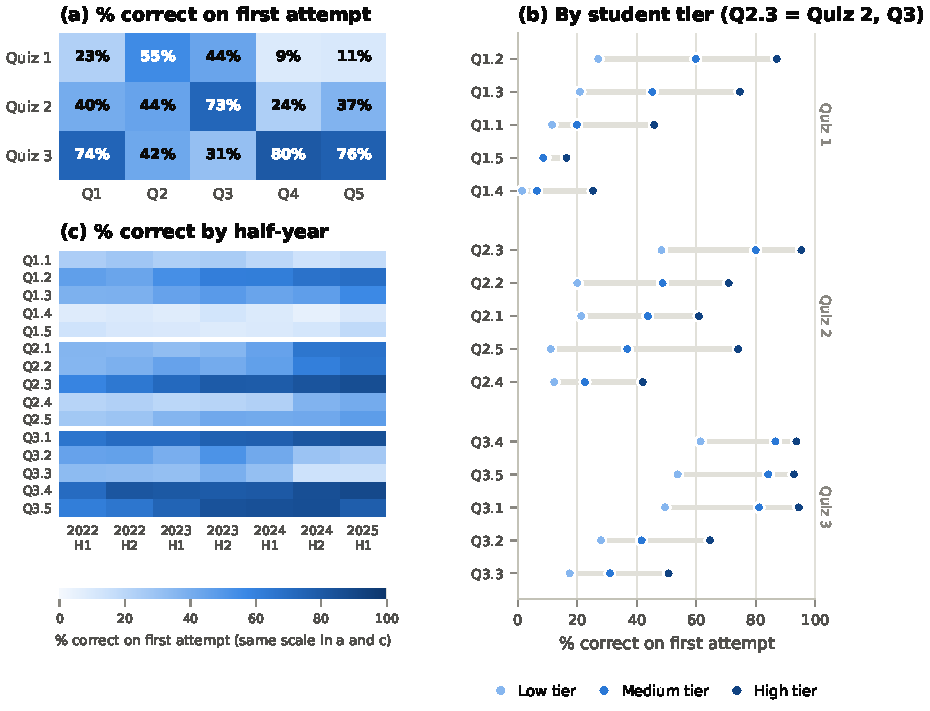
\includegraphics[width=\linewidth]{fig03_h2_question_difficulty.pdf}
\caption{H2. (a) Facility index (\% correct on first attempt) for each
question. (b) Facility by student tier; questions are sorted from easiest to
hardest within each quiz. (c) Facility for each half-year, same colour
scale as (a).}
\label{fig:h2}
\end{figure}

\begin{mctable}
(a), (c) cells & Area (rectangle) & Colour lightness (sequential blue) $\rightarrow$ \% correct; row/column position $\rightarrow$ quiz--question / half-year; text $\rightarrow$ exact value in (a) \\
(b) tier values & Point & Horizontal position $\rightarrow$ \% correct; vertical position $\rightarrow$ question; lightness of blue $\rightarrow$ tier (ordered) \\
(b) range & Line & Length $\rightarrow$ gap between tiers \\
\end{mctable}

\textbf{What we see.} The differences are large. Inside Quiz 1 the facility
goes from 55\% (Q1.2) down to 9\% (Q1.4) and 10\% (Q1.5). In Quiz 2 it goes
from 73\% (Q2.3) to 24\% (Q2.4), and in Quiz 3 from 80\% (Q3.4) to 31\%
(Q3.3). A chi-square test confirms that the questions inside each quiz are not
equally hard ($p < 0.001$, Cram\'er's $V$ = 0.33--0.41, a large effect).

The ranking is also stable. In panel (b), the hardest questions sit at the
bottom of their quiz for \emph{every} tier: even High-tier students get only
25\% of Q1.4 and 16\% of Q1.5 right, and Q3.3 is the hardest question in Quiz 3
for all three tiers. In panel (c) the rows keep their shade over time. The
hardest question in each quiz was the hardest in 6 of 7 half-years for Quiz 1
and in 7 of 7 for Quizzes 2 and 3. Kendall's $W$, which measures how much the
rankings agree across half-years, is 0.95, 0.85 and 0.87 (1 means perfect
agreement). Panel (c) also shows a few real changes, for example Q2.1 and Q2.2
became easier and Q3.2 and Q3.3 became harder in the second half of 2024. We
come back to this in H9.

\begin{decision}
\textbf{Decision: \accepted.} Some questions are much harder than others
(e.g.\ Q1.4 at 9\% vs.\ Q1.2 at 55\%), and the same questions stay hard for
weak and strong students and across three years.
\end{decision}

% ............................................................ H3
\subsubsection{H3 -- Do high performers improve steadily and low performers erratically?}
\label{sec:h3}

\begin{hyp}{H3}
High-performing students consistently improve scores over multiple attempts,
whereas low performers show erratic progress.
\end{hyp}

\textbf{How we tested it.} We took every student--quiz pair with at least two
attempts (8,130 pairs) and looked at how the grade changed from one attempt to
the next. We measured ``consistent improvement'' by the share of re-attempts
that went up, and ``erratic progress'' by the share of students (with three or
more attempts) whose grade dropped at least once.

There is a trap here. If tiers are defined using the same marks we are
studying, students put in the Low tier because of a bad first attempt will
improve partly by chance (regression to the mean, \citet{barnett2005regression}).
To check this, we repeated the analysis with a second tier definition that uses
\emph{only the other two quizzes} to decide a student's level.

\textbf{Why this chart.} Panel (a) is a line chart because attempt number is
ordered, and lines show the direction of change clearly; the shaded band is the
95\% confidence interval. Panel (b) uses 100\% stacked bars with a diverging
colour scale (red = down, grey = same, blue = up), so the share of each
direction can be read as a length and the ``bad'' and ``good'' sides are easy
to tell apart. Panel (c) uses dots with confidence intervals, and two shapes for
the two tier definitions, so the extra check sits right next to the main
result.

\begin{figure}[H]
\centering
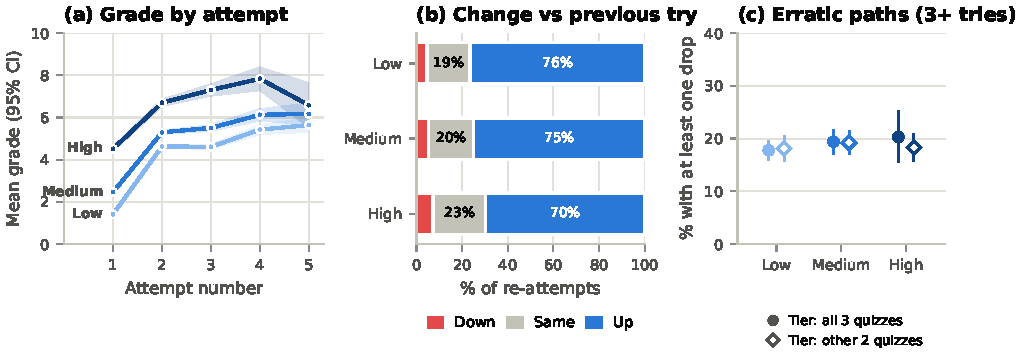
\includegraphics[width=\linewidth]{fig04_h3_progress_by_tier.pdf}
\caption{H3. (a) Mean grade by attempt number for each tier (students with 2+
attempts). (b) Direction of change from the previous attempt. (c) Share of
students with 3+ attempts whose grade dropped at least once; circles use the
normal tier, hollow diamonds use a tier based only on the other two quizzes.}
\label{fig:h3}
\end{figure}

\begin{mctable}
(a) mean grade & Point + line & Vertical position $\rightarrow$ mean grade; horizontal position $\rightarrow$ attempt number; lightness $\rightarrow$ tier \\
(a) uncertainty & Area & Band height $\rightarrow$ 95\% CI \\
(b) change & Line (bar segment) & Length $\rightarrow$ share of re-attempts; diverging hue $\rightarrow$ down / same / up \\
(c) erratic share & Point + error bar & Vertical position $\rightarrow$ \% with a drop; shape and fill $\rightarrow$ tier definition \\
\end{mctable}

\textbf{What we see.} All three tiers improve, and they improve in the same
way. In panel (b), 76\% of Low-tier re-attempts went up and only 5\% went down;
for High-tier students it was 70\% up and 7\% down. Low performers actually
gained the most from first to last attempt (+4.7 marks on average, against
+3.0 for High performers), because they started lower. Panel (c) shows that
``erratic'' paths are equally common in every tier: 18\% of Low, 19\% of Medium
and 20\% of High students with three or more attempts had at least one drop,
and the confidence intervals overlap. The hollow diamonds (tier from the other
two quizzes) give almost the same values (18\%, 19\%, 18\%), so the result is
not caused by regression to the mean.

The more useful explanation comes from H6: students mostly keep trying until
they pass and then stop, which makes almost everyone's path go up in the same
way.

\begin{decision}
\textbf{Decision: \rejected.} High performers do improve, but so do low
performers, and low performers are not more erratic. The share of drops is
about 5--7\% of re-attempts in every tier, and about 18--20\% of students with
3+ attempts in every tier.
\end{decision}

% ............................................................ H4
\subsubsection{H4 -- Do hard questions take longer, and are strong students faster on them?}
\label{sec:h4}

\begin{hyp}{H4}
More difficult questions take longer to answer, but higher-performing students
answer them faster than lower-performing students.
\end{hyp}

\textbf{An important limitation.} The data only gives the time for the
\emph{whole attempt}, not for each question. So this hypothesis cannot be
tested directly. We used two indirect tests instead.

\begin{enumerate}
  \item \textbf{Part 1, indirect test.} If a question needs more thinking time,
        then students who got it \emph{right} should have spent more time on the
        attempt than students who got it wrong, and this gap should be bigger
        for harder questions. For each of the 15 questions we calculated the
        ratio \emph{median time when correct $\div$ median time when wrong}
        (first attempts) and plotted it against the facility index.
  \item \textbf{Part 2, indirect test.} For the hardest question in each quiz,
        we took only the first attempts that got it right and compared the time
        taken by Low, Medium and High tier students.
\end{enumerate}

\textbf{Why this chart.} Part 1 compares two numeric values for 15 items, so a
labelled scatter plot is the natural choice; a horizontal reference line at 1
marks ``no time difference'' and a light trend line helps the eye. Part 2
compares a median between ordered groups, so we used dots with bootstrap
confidence intervals instead of bars, which would suggest a quantity that
starts from zero. Sample sizes are printed under each dot, because one group is
small.

\begin{figure}[H]
\centering
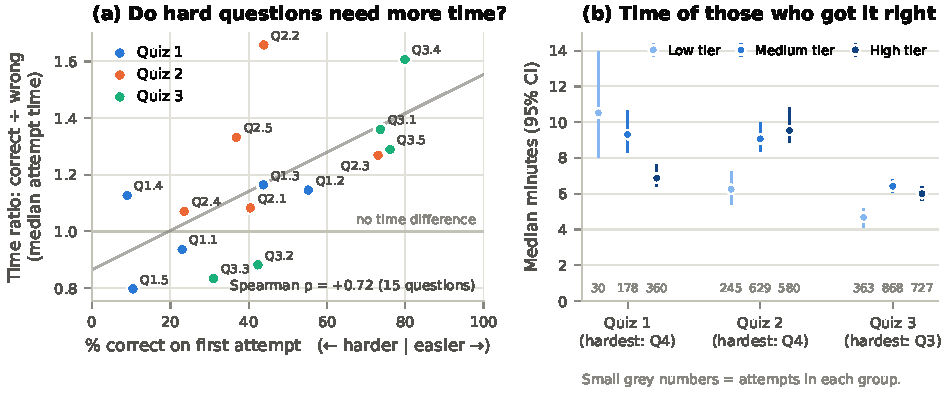
\includegraphics[width=\linewidth]{fig05_h4_difficulty_speed.pdf}
\caption{H4. (a) For each question: facility index vs.\ how much longer the
attempt took when the question was answered correctly. Points above 1 mean
correct answers came with more time. (b) Median time of first attempts that
answered the hardest question correctly, by tier, with 95\% bootstrap CIs.}
\label{fig:h4}
\end{figure}

\begin{mctable}
(a) question & Point & Horizontal position $\rightarrow$ facility index; vertical position $\rightarrow$ time ratio; hue $\rightarrow$ quiz; text $\rightarrow$ question ID \\
(a) reference & Line & Position $\rightarrow$ ratio of 1 (no difference) and linear trend \\
(b) tier medians & Point + error bar & Vertical position $\rightarrow$ median minutes; horizontal position $\rightarrow$ quiz and tier; lightness $\rightarrow$ tier \\
\end{mctable}

\textbf{What we see.} In panel (a) the points go \emph{up} to the right
(\rhoeq{+0.72}, $p = 0.003$). This is the opposite of Part 1: the time
``reward'' for getting a question right is biggest for \emph{easy} questions
(e.g.\ Q3.4 at 80\% facility, ratio 1.61) and smallest, or even below 1, for
hard ones (Q1.5 at 0.80, Q3.3 at 0.83). In other words, students who solve the
hardest questions do not seem to spend extra time on them. The quiz level gives
the same message: the hardest quiz (Quiz 1, mean 2.8/10) is not the slowest;
Quiz 2 is (median 8.4 minutes vs.\ 7.1 for Quiz 1).

Panel (b) supports Part 2 only in Quiz 1, where High-tier students who solved
Q1.4 needed 6.9 minutes against 9.3 for Medium and 10.5 for Low (but only 30
Low-tier students solved it). In Quiz 2 and Quiz 3 the result is reversed: the
Low tier was the \emph{fastest} (6.3 and 4.7 minutes). This matches a wider
pattern in the data: on first attempts, Low-tier students are the fastest in
all three quizzes (median 6.1, 6.3 and 5.1 minutes, against 7.3, 9.2 and 7.0
for the High tier). They seem to rush rather than to struggle.

\begin{decision}
\textbf{Decision: \rejected{} (with an important limitation).} Within what
the data allows us to test, hard questions do not go with longer times, and
higher-performing students are not generally faster; low performers are
usually the fastest. Because per-question times are not recorded, this is an
indirect test and the hypothesis should be re-checked with per-question time
logs.
\end{decision}

% ............................................................ H5
\subsubsection{H5 -- Is there an optimal time range?}
\label{sec:h5}

\begin{hyp}{H5}
There is an optimal time range for achieving higher scores, and students who
finish too quickly or take too long tend to score lower.
\end{hyp}

\textbf{How we tested it.} We grouped first attempts into time bins (from under
1 minute to over 1 day) and plotted the mean grade for each bin, per quiz. Here
we \emph{kept} the attempts over 60 minutes, because ``taking too long'' is part
of the hypothesis. We marked the best bin under one hour for each quiz.

\textbf{Why this chart.} An inverted-U shape is a question about the
\emph{shape} of a trend, which a line chart shows best. The x-axis is on a log
scale so that the short times, where most attempts are, get enough space. The
grey shaded area marks attempts over one hour, so readers know those times are
probably not real working time. The number of attempts per bin is shown in a
second, aligned panel instead of on a second y-axis, which would invite false
comparisons between the two scales.

\begin{figure}[H]
\centering
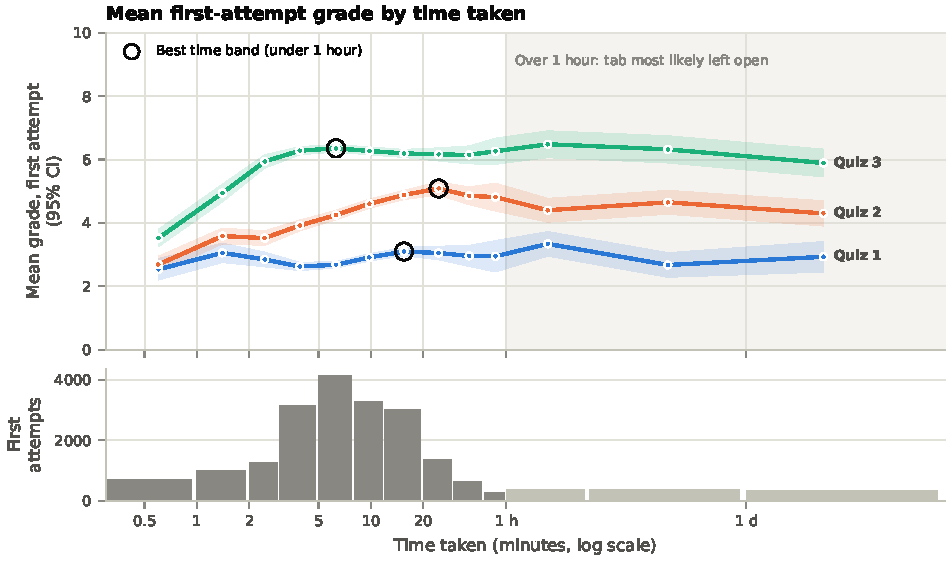
\includegraphics[width=\linewidth]{fig06_h5_optimal_time.pdf}
\caption{H5. Top: mean first-attempt grade by time bin with 95\% CI; circles
mark each quiz's best bin under one hour. Bottom: number of first attempts in
each bin. Bins: $<$1, 1--2, 2--3, 3--5, 5--8, 8--12, 12--20, 20--30, 30--45,
45--60 min, 1--3 h, 3--24 h, $>$1 day.}
\label{fig:h5}
\end{figure}

\begin{mctable}
Mean grade per bin & Point + line & Vertical position $\rightarrow$ mean grade; horizontal position (log) $\rightarrow$ time bin; hue $\rightarrow$ quiz \\
Uncertainty & Area & Band height $\rightarrow$ 95\% CI \\
Best bin & Point (ring) & Shape $\rightarrow$ ``best time band'' \\
Over 1 hour & Area (background) & Grey shade $\rightarrow$ probably idle time \\
Counts & Line (bar) & Length $\rightarrow$ number of attempts \\
\end{mctable}

\textbf{What we see.} The ``too fast'' part is very clear. First attempts
finished in under a minute score far lower: 2.5, 2.7 and 3.5 in Quizzes 1, 2
and 3, which is 1.6 marks below the quiz average when the quizzes are combined.
Scores rise quickly over the first few minutes and then level off. The best
band is different for each quiz: 5--8 minutes for Quiz 3 (6.35), 12--20 minutes
for Quiz 1 (3.10) and 20--30 minutes for Quiz 2 (5.09). After the peak the
lines go down only a little. Attempts left open for more than a day score
about the same as the quiz average (0.05 below), which is about 0.4 marks
below the peak. A simple curve fitted to all first attempts under an hour has
its peak at about 25 minutes. So there is a strong ``too fast'' penalty but
only a small ``too slow'' penalty, and the shape is more of a rise followed by a
plateau than a sharp peak. For Quiz 1, the hardest quiz, time hardly matters at
all.

\begin{decision}
\textbf{Decision: \partly.} Finishing too quickly clearly goes with lower
scores, and each quiz has a best time band. But taking too long has only a
small effect, so the ``inverted U'' is weak on the right side, and the best
band is not the same for every quiz.
\end{decision}

% ---------------------------------------------------------------- Task 2
\subsection{Task 2: our own hypotheses}

While exploring the data for Task 1 we noticed some patterns that the given
hypotheses did not cover: almost nobody stopped with a grade below 4, some
re-attempts took under a minute and got full marks, and two questions were often
left blank. We built our five hypotheses around these observations and around
ideas from the literature in Section~\ref{sec:background}. We also chose
hypotheses that need different kinds of charts, so that together they show
different parts of the data.

% ............................................................ H6
\subsubsection{H6 -- Do students re-attempt to pass, not to get full marks?}
\label{sec:h6}

\begin{hyp}{H6}
Students re-attempt a quiz mainly to reach a pass mark. Once they reach it,
most of them stop, even if they could still improve.
\end{hyp}

\textbf{How we tested it.} For every finished attempt we checked whether the
same student made another attempt on the same quiz. We then compared this
``try again'' rate across grades. If H6 is true, the rate should drop
sharply at one grade (the pass mark), not slowly as the grade goes up. We also
looked at where re-attempting students finally stopped.

\textbf{Why this chart.} Panel (a) uses grouped bars because we are comparing
a \emph{proportion} (which starts at zero) across ordered grades and three
quizzes; the shaded background marks grades below 4. Panel (b) uses 100\%
stacked bars with an ordered light-to-dark scale, which shows a
part-to-whole split of final grades and lets us compare two groups on the same
length scale. We did not use pie charts because two pies are hard to compare.

\begin{figure}[H]
\centering
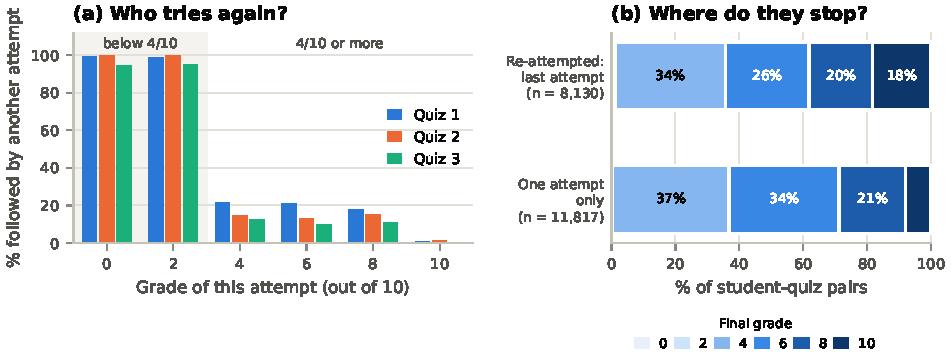
\includegraphics[width=\linewidth]{fig07_h6_pass_mark.pdf}
\caption{H6. (a) Share of attempts that were followed by another attempt on the
same quiz, by grade. (b) Final grade of students who re-attempted (their last
attempt) compared with students who made only one attempt.}
\label{fig:h6}
\end{figure}

\begin{mctable}
(a) re-attempt rate & Line (bar) & Length / vertical position $\rightarrow$ \% followed by another attempt; horizontal position $\rightarrow$ grade; hue $\rightarrow$ quiz \\
(a) fail zone & Area (background) & Grey shade $\rightarrow$ grades below 4 \\
(b) final grade split & Line (bar segment) & Length $\rightarrow$ share; lightness (ordered blue) $\rightarrow$ final grade \\
\end{mctable}

\textbf{What we see.} Panel (a) shows a cliff, not a slope. After a grade of 0
or 2, students tried again 98.7\% of the time. After a grade of 4, 6 or 8 the
rate falls to only 15.6\%, and after 10 it is 0.8\%. The drop happens exactly
between 2 and 4 in all three quizzes, and the rates for 4, 6 and 8 are almost
the same, so it is not simply ``the higher the grade, the less need to retry''.
The split is very strong (Cram\'er's $V$ = 0.78). Panel (b) shows where
students stop: 34.5\% of re-attempting students stopped at exactly 4/10, and
only 18\% went on to full marks. Among the 11,817 student--quiz pairs with only
one attempt, just 25 had a grade below 4. Together this strongly suggests that
the course uses 4/10 (40\%) as the pass mark, and that students treat it as the
goal. This is a clear example of satisficing \citep{simon1956rational}.

\begin{decision}
\textbf{Decision: \accepted.} Students below 4/10 almost always try again;
students at 4/10 or above almost always stop, and about a third of re-attempters
stop exactly at 4. Re-attempts are used to pass, not to master the material.
\end{decision}

% ............................................................ H7
\subsubsection{H7 -- Do instant re-attempts reuse the feedback?}
\label{sec:h7}

\begin{hyp}{H7}
When students are allowed to re-attempt immediately, the re-attempt gives a much
larger gain (they reuse the answers they have just seen in the feedback). When
there is a waiting time between attempts, this effect disappears.
\end{hyp}

\textbf{How we found it.} In H1 we saw re-attempts with full marks in about a
minute. To understand them we plotted the waiting time before every re-attempt
against the date. This showed something we did not expect: up to 12 May 2022
many re-attempts started within a minute of the previous one, but from 13 May
2022 \emph{no} re-attempt starts less than 120 minutes after the previous
attempt ended. The minimum waiting time after that date is exactly 120 minutes.
This looks like Moodle's ``enforced delay between attempts'' setting being
switched on with a value of 2 hours \citep{moodle_settings}. It gives us a
natural experiment: the same quizzes, before and after a waiting time was
added.

\textbf{Why this chart.} Panel (a) is a scatter plot because we want to see
every individual re-attempt and spot a sudden change; the y-axis is on a log
scale because waiting times go from seconds to months. We used colour for
\emph{emphasis}: re-attempts with 10/10 are orange and everything else is grey,
so the cluster of perfect, instant re-attempts stands out. Panel (b) uses 100\%
stacked bars to compare the grade distribution of three groups of re-attempts
on one length scale, with the sample size and the mean gain written above each
bar.

\begin{figure}[H]
\centering
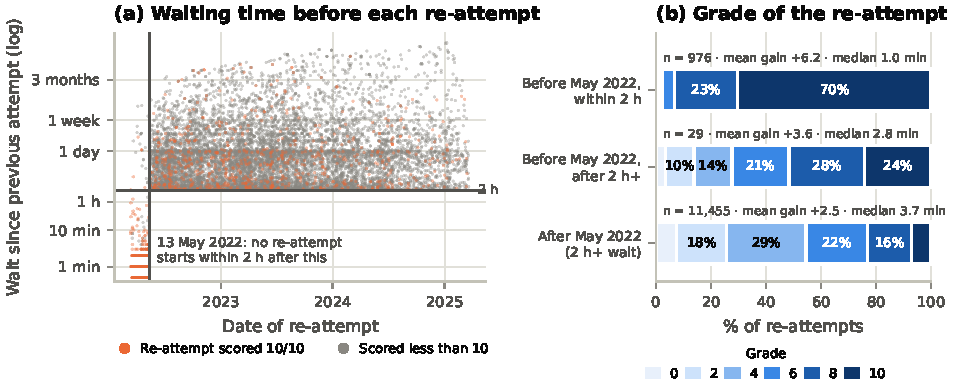
\includegraphics[width=\linewidth]{fig08_h7_retake_delay.pdf}
\caption{H7. (a) Waiting time before each of the 12,460 re-attempts, by date
(log scale). Orange = re-attempt scored 10/10. (b) Grade of the re-attempt for
three groups: before 13 May 2022 within 2 hours, before 13 May 2022 after 2+
hours, and after 13 May 2022 (always 2+ hours).}
\label{fig:h7}
\end{figure}

\begin{mctable}
(a) each re-attempt & Point & Horizontal position $\rightarrow$ date; vertical position (log) $\rightarrow$ waiting time; hue (orange vs.\ grey) $\rightarrow$ full marks or not \\
(a) reference & Line & Position $\rightarrow$ 2-hour floor and change date \\
(b) grade split & Line (bar segment) & Length $\rightarrow$ share of re-attempts; lightness (ordered blue) $\rightarrow$ grade; vertical position $\rightarrow$ group \\
\end{mctable}

\textbf{What we see.} Before the change, 976 of the 1,005 re-attempts started
within two hours, most of them within a minute. These quick re-attempts scored
9.2/10 on average, 70\% got full marks, and the median attempt took only 1.0
minute. The average gain over the previous attempt was +6.2 marks. After the
change, the average gain fell to +2.5 marks, only 7\% of re-attempts got full
marks, and the median time went up to 3.7 minutes. The difference in gains is
very large (Mann--Whitney $p < 0.001$; a random quick re-attempt gains more than
a random later one 84\% of the time). The earlier students were not stronger: their
previous grade was similar (3.0 vs.\ 2.4 on average), and their first-attempt
grades were in fact lower (3.7 vs.\ 4.5). A five-question
quiz cannot honestly be read and answered in one minute
\citep{wise2005response}, so the most likely explanation is that students were
copying the correct answers shown in the review of the previous attempt, a form
of ``gaming the system'' \citep{baker2004offtask, alexandron2017copying}.

The 29 re-attempts before May 2022 that did wait two hours or more gained +3.6
on average, between the two other groups. This group is small, so we do not
read much into it.

\begin{decision}
\textbf{Decision: \accepted.} Instant re-attempts gave very large, very fast
gains (+6.2 marks in about a minute, 70\% full marks). Once a two-hour wait was
enforced, these disappeared (+2.5 marks, 7\% full marks). This also explains
the fast, high-scoring re-attempts in H1 and H5.
\end{decision}

% ............................................................ H8
\subsubsection{H8 -- Does a good Quiz 1 result carry over to later quizzes?}
\label{sec:h8}

\begin{hyp}{H8}
Students who do well on Quiz 1 also do well on Quiz 2 and Quiz 3.
\end{hyp}

\textbf{How we tested it.} We used each student's \emph{first-attempt} grade on
each quiz (6,635 students who finished all three) and put it into three bands:
0--2 (failed), 4 (just passed) and 6--10 (good). We then followed each student
across the quizzes. We also computed Spearman's $\rho$ between the raw grades.

\textbf{Why this chart.} We want to see how groups of students \emph{move}
between bands over three steps. An alluvial diagram is made for this
\citep{rosvall2010mapping}: the blocks show how big each band is in each quiz,
and the ribbons show how many students move from one band to another. We
coloured every ribbon by the student's band in Quiz 1, so a reader can follow,
for example, the dark ``good in Quiz 1'' group all the way to Quiz 3. Panel (b)
then gives one clear number per Quiz 1 band using a bar chart with confidence
intervals, because the alluvial diagram is good for an overview but not for
reading exact values.

\begin{figure}[H]
\centering
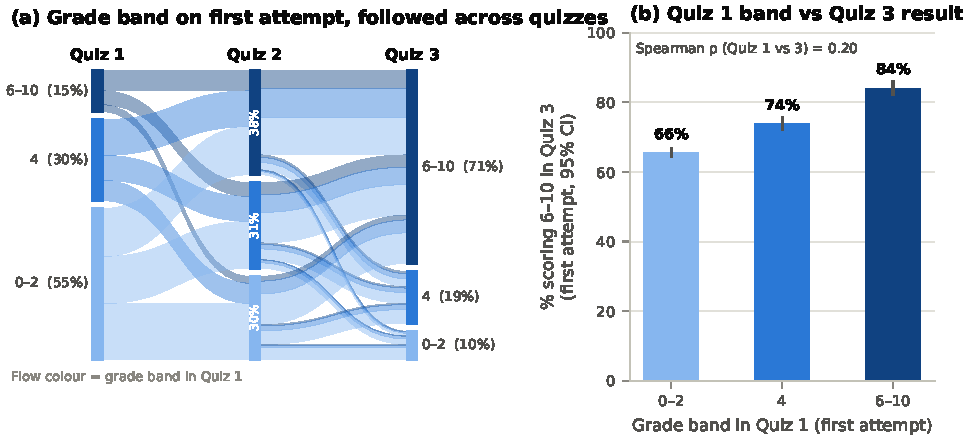
\includegraphics[width=\linewidth]{fig09_h8_carry_over.pdf}
\caption{H8. (a) Alluvial diagram of first-attempt grade bands across the three
quizzes; ribbon colour = band in Quiz 1. (b) Share of students who scored 6--10
on their first attempt in Quiz 3, by their band in Quiz 1.}
\label{fig:h8}
\end{figure}

\begin{mctable}
(a) band block & Area (rectangle) & Vertical length $\rightarrow$ share of students; horizontal position $\rightarrow$ quiz; vertical position $\rightarrow$ band (ordered); lightness $\rightarrow$ band \\
(a) ribbon & Area (flow) & Width $\rightarrow$ number of students moving; lightness $\rightarrow$ band in Quiz 1 \\
(b) outcome & Line (bar) + error bar & Length $\rightarrow$ \% scoring 6--10 in Quiz 3; lightness $\rightarrow$ Quiz 1 band \\
\end{mctable}

\textbf{What we see.} The direction is as expected: 84\% of students who scored
6--10 in Quiz 1 also scored 6--10 in Quiz 3, compared with 74\% of those who
scored 4 and 66\% of those who scored 0--2. But the alluvial diagram mostly
shows a lot of \emph{mixing}. Many students who failed Quiz 1 at first are in
the top band of Quiz 3, and only 43\% of the students in the top band of Quiz 1
stayed in the top band for both later quizzes. The correlation between
first-attempt grades is weak for every pair of quizzes ($\rho$ = 0.20 for
Quiz 1--2, 0.20 for 1--3 and 0.21 for 2--3; Cram\'er's $V$ = 0.11). One reason
is that the quizzes are very different in difficulty (Figure~\ref{fig:overview}c),
but even inside the same quiz the ranking of students changes a lot.

\begin{decision}
\textbf{Decision: \partly.} The direction is right (good in Quiz 1 $\rightarrow$
more likely to be good in Quiz 3), but the link is weak ($\rho \approx 0.2$).
A student's Quiz 1 result is a poor predictor of how they will do later, so
teachers should not label students early based on Quiz 1.
\end{decision}

% ............................................................ H9
\subsubsection{H9 -- Did later groups of students do better?}
\label{sec:h9}

\begin{hyp}{H9}
Students who took the quizzes later (2024--2025) score higher on their first
attempt than students who took them earlier (2022).
\end{hyp}

\textbf{How we tested it.} We grouped students into \emph{cohorts} by the
half-year of their first attempt on each quiz, and plotted the mean
first-attempt grade and the share of students who needed a re-attempt for
each cohort.

\textbf{Why this chart.} Cohorts are ordered in time, so a line chart is the
best fit; the lines are labelled directly at their ends, so no legend is
needed, and the 95\% confidence bands show which changes are bigger than the
noise. We put the grade and the re-attempt share in two separate panels instead
of one chart with two y-axes, because they are on different scales.

\begin{figure}[H]
\centering
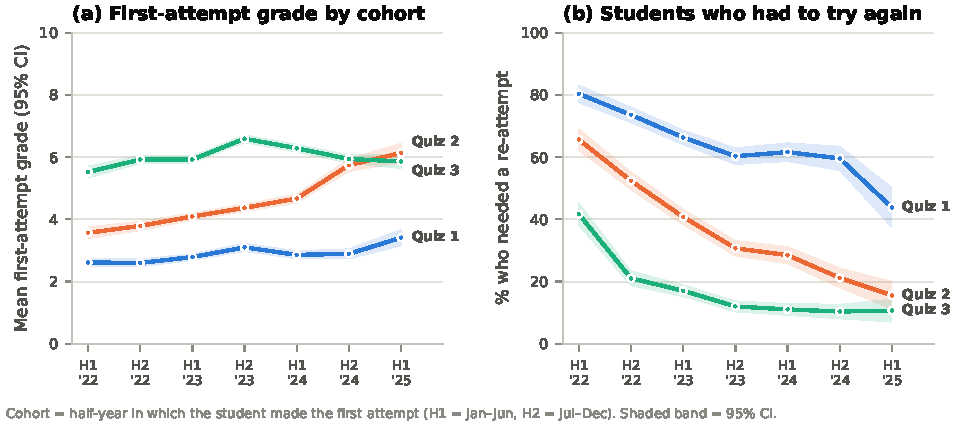
\includegraphics[width=\linewidth]{fig10_h9_cohort_trend.pdf}
\caption{H9. (a) Mean first-attempt grade by cohort (half-year). (b) Share of
students in each cohort who made more than one attempt.}
\label{fig:h9}
\end{figure}

\begin{mctable}
Cohort value & Point + line & Vertical position $\rightarrow$ mean grade or \% re-attempting; horizontal position $\rightarrow$ half-year (ordered); hue $\rightarrow$ quiz \\
Uncertainty & Area & Band height $\rightarrow$ 95\% CI \\
\end{mctable}

\textbf{What we see.} The three quizzes behave differently. Quiz 2 shows a big
and steady rise, from a mean of 3.6 in the first half of 2022 to 6.1 in early
2025 (\rhoeq{0.24}), with a jump in the second half of 2024. Quiz 1 rises only a
little, from 2.6 to 3.4 (\rhoeq{0.08}). Quiz 3 goes up until 2023 and then
comes back down (5.5, 6.6, then 5.9), so it has no clear trend. In panel (b)
the share of students who needed a re-attempt falls in all three quizzes (Quiz
1: 80\% to 44\%; Quiz 2: 66\% to 16\%; Quiz 3: 42\% to 11\%). Part of this fall
is caused by fewer students failing, and part by the two-hour delay from H7:
after it was introduced, far fewer students who had already passed tried again
just to improve.

We cannot say for sure \emph{why} Quiz 2 got easier. Figure~\ref{fig:h2}c shows
that Q2.1 and Q2.2 became much easier at the same time (from 45\% to 65\% and
from 46\% to 61\% between the two halves of 2024) while Q3.2 and Q3.3 became
harder. Changes this sudden look more like edits to the questions than a slow
change in students. Answers being shared between cohorts is another
possibility. Also, students in the last half-year had less time before the data
was exported, so their re-attempt share may be slightly too low.

\begin{decision}
\textbf{Decision: \partly.} Later cohorts did clearly better in Quiz 2, a
little better in Quiz 1, and not better in Quiz 3. Fewer students needed a
re-attempt in every quiz.
\end{decision}

% ............................................................ H10
\subsubsection{H10 -- Is a blank answer a sign of low effort?}
\label{sec:h10}

\begin{hyp}{H10}
Leaving a question blank is a sign of low effort: attempts with a blank answer
are finished faster and also score lower on the questions that were answered.
\end{hyp}

\textbf{How we tested it.} Only two questions are left blank often: Q1.4 (9.0\%
of first attempts) and Q2.5 (9.1\%). For these two, we compared first attempts
where the question was left blank with those where it was answered, on three
things: time taken, marks on the \emph{other four} questions (so the blank
itself does not count) and the share of attempts made by Low-tier students.

\textbf{Why this chart.} Time is skewed, so panel (a) uses box plots on a log
scale, which show the median and spread rather than a single average. Panels
(b) and (c) compare a mean and a proportion between two groups. The same layout
is used in all three panels, with hollow marks for ``answered'' and filled marks
for ``blank'', so the eye can move across the panels and read the same contrast
three times. Quiz colours stay the same as in all other figures.

\begin{figure}[H]
\centering
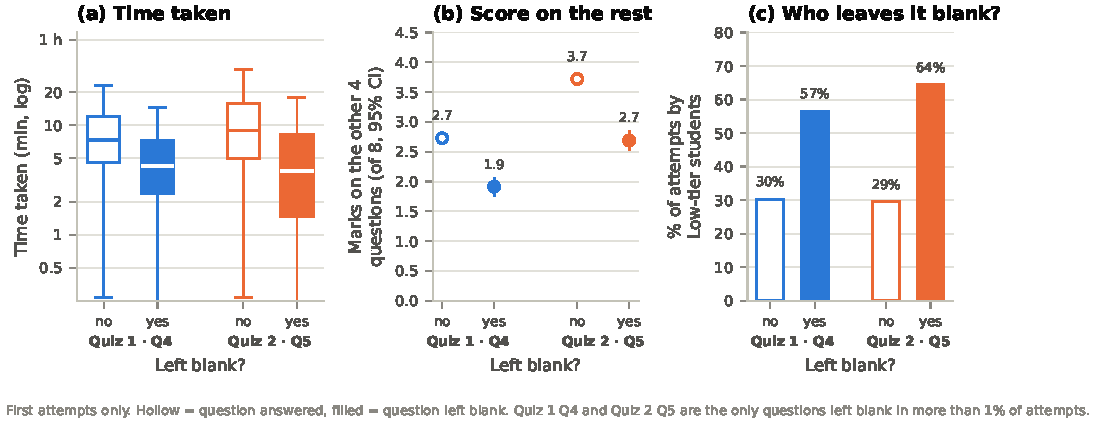
\includegraphics[width=\linewidth]{fig11_h10_blank_answers.pdf}
\caption{H10. First attempts for the two questions that are often left blank.
(a) Time taken. (b) Marks on the other four questions (out of 8) with 95\% CI.
(c) Share of these attempts made by Low-tier students.}
\label{fig:h10}
\end{figure}

\begin{mctable}
(a) time & Box plot (lines + area) & Vertical position (log) $\rightarrow$ median, quartiles and range of time \\
(b) other marks & Point + error bar & Vertical position $\rightarrow$ mean marks on other questions \\
(c) Low-tier share & Line (bar) & Length $\rightarrow$ \% Low-tier \\
All panels & -- & Fill (hollow vs.\ filled) $\rightarrow$ answered vs.\ blank; hue $\rightarrow$ quiz \\
\end{mctable}

\textbf{What we see.} All three panels tell the same story. Attempts that left
Q1.4 blank took a median of 4.3 minutes against 7.3 minutes for those that
answered it, and for Q2.5 it was 3.8 against 8.9 minutes. One in five (20\%) of
the Q1.4 blanks and 30\% of the Q2.5 blanks were finished in under two minutes,
compared with 6\% and 8\% of the others. These students also scored lower on
the questions they \emph{did} answer: 1.9 vs.\ 2.7 out of 8 in Quiz 1, and 2.7
vs.\ 3.7 in Quiz 2 (both $p < 0.001$). More than half of the blank attempts
came from Low-tier students (57\% and 64\%), against about 30\% of the answered
ones. The blank rate also falls steadily with tier: 15.5\% of Low, 7.4\% of
Medium and 2.5\% of High students left Q1.4 blank. This fits the idea of rapid,
low-effort responding described by \citet{wise2005response}.

\begin{decision}
\textbf{Decision: \accepted.} Attempts with a blank answer were about twice as
fast and scored lower on the other questions, and they came mostly from
low-performing students. A blank answer is a useful, cheap warning sign of low
effort.
\end{decision}


% ================================================================== 6
\section{Discussion}
\label{sec:discussion}

\subsection{Putting the results together}

Looking at the ten results side by side, one message stands out: \textbf{the
rules of the quiz shape student behaviour more than the time they spend.} Two
rules explain a lot of what we saw.

\begin{itemize}
  \item \textbf{The pass mark (H6).} Students keep trying until they reach
        4/10 and then stop. This is why almost every re-attempt path goes up,
        for weak and strong students alike (H3), and why so many students end
        at exactly 4.
  \item \textbf{The attempt delay (H7).} While re-attempts were allowed
        straight away, students could copy the answers they had just seen and
        get full marks in about a minute. These fast, perfect re-attempts are
        what flips the time--score relationship in H1, and they made ``very
        fast'' attempts look good when all attempts were mixed together.
\end{itemize}

A second message is that \textbf{speed means different things for different
students}. Strong students are not faster on hard questions (H4). It is the
weaker students who are fastest, and they are also the ones who leave questions
blank (H10) and finish in under a minute with low marks (H5). This matches the
idea of rapid, low-effort responding \citep{wise2005response} more than the
idea of slow, struggling students. It also fits the finding of
\citet{goldhammer2014time} that the meaning of time on task depends on the
person and the task.

The most stable thing in the data is \textbf{question difficulty} (H2). The
same questions are hard for every tier and in almost every half-year. The few
clear changes (for example in mid-2024 in Quizzes 2 and 3) are sudden, which
suggests the questions themselves were edited (H9).

Finally, \textbf{a single quiz is a weak signal of a student's level} (H8).
First-attempt grades in different quizzes are only weakly related
($\rho \approx 0.2$). Part of this is because the quizzes cover different
material and have very different difficulty, but it is also a reminder that
five two-mark questions give a noisy measure.

\subsection{What a teacher could do with these results}

\begin{enumerate}
  \item \textbf{Keep the enforced delay between attempts.} H7 shows it removed
        most of the ``copy the feedback'' behaviour. Showing the correct
        answers only after the quiz closes, or drawing each re-attempt from a
        pool of question variants, would make re-attempts even more useful.
  \item \textbf{Review Q1.4, Q1.5 and Q3.3.} Only 9--31\% of students get
        these right on the first try. Q1.5 is a special case: even High-tier
        students get it right only 16\% of the time, against 9\% for Low-tier
        students (Figure~\ref{fig:h2}b). A question that strong and weak
        students fail almost equally often does not separate them, and Moodle's
        own guidance says this can be a sign of a wrong answer key or unclear
        wording \citep{moodle_stats}.
  \item \textbf{Think about the pass mark.} If the goal is mastery, a pass mark
        of 4/10 may be too low, because most students stop there (H6). A
        higher threshold, or a small reward for reaching 8 or 10, could change
        this.
  \item \textbf{Use cheap warning signs.} A blank answer, or a first attempt
        under one minute, are easy to detect and are strongly linked to low
        performance (H5, H10). They could trigger a friendly message or extra
        support.
  \item \textbf{Do not judge students on Quiz 1 alone} (H8).
\end{enumerate}

\subsection{Reflection on our visualization choices}

Table~\ref{tab:vischoices} summarises the main chart used for each hypothesis.
A few lessons came out of the process.

\begin{itemize}
  \item \textbf{Our first idea was not always the right one.} For H1 we first
        drew a scatter plot of time against grade. With 30,000 points and only
        six grades it became six solid stripes and showed nothing. Replacing it
        with medians and IQR bars, split by attempt type, showed the real
        pattern, including the reversal.
  \item \textbf{Splitting the data was more important than the chart type.}
        Separating first attempts from re-attempts, and showing the quizzes
        separately, changed the answers to H1 and H5.
  \item \textbf{Highlighting one thing can reveal a story.} In H7, colouring
        only the full-mark re-attempts and greying the rest made the cluster of
        instant perfect re-attempts, and the sudden two-hour floor, visible at a
        glance. We would not have found the change in the quiz settings from a
        table.
  \item \textbf{We avoided some common mistakes on purpose:} no pie charts, no
        dual y-axes, no rainbow colour scales, no 3D. Where we needed both a
        trend and the number of cases (H5), we used two aligned panels.
\end{itemize}

\begin{table}[H]
\centering
\small
\caption{Summary of the main visualization for each hypothesis.}
\label{tab:vischoices}
\begin{tabularx}{\linewidth}{@{}l >{\raggedright\arraybackslash}p{2.6cm} >{\raggedright\arraybackslash}p{3.5cm} X@{}}
\toprule
\textbf{H} & \textbf{Chart} & \textbf{Main marks \& channels} & \textbf{Why this and not something else} \\
\midrule
H1 & Median + IQR dot-line, 2 panels & Points/lines; y-position (log time), x-position (grade), hue (quiz) & A scatter plot of 30k points on 6 grade values overplots; medians show the trend and IQR shows spread. \\
H2 & Heatmaps + tier dot plot & Cells with lightness + labels; points on a common x-scale & Heatmap gives an overview of 15 or 105 values; dot plot gives accurate tier comparison. \\
H3 & Line + CI, stacked bars, dot + CI & Lines (position), diverging hue for up/down, shape for tier method & Attempt number is ordered; diverging colours separate good and bad changes; two shapes show the extra check. \\
H4 & Labelled scatter; dot + bootstrap CI & Points: x = facility, y = time ratio, hue = quiz & Two numeric values for 15 items; medians with CIs, not bars, for skewed time. \\
H5 & Line + CI band, aligned count panel & Lines; x-position (log time bins), y-position (mean grade) & Shape of a trend needs a line; aligned panel instead of a dual axis. \\
H6 & Grouped bars; 100\% stacked bars & Length (proportion), ordered lightness & Proportions start at zero, so bars are correct; stacked bars compare two distributions better than pies. \\
H7 & Scatter over time (emphasis colour); stacked bars & Points: x = date, y = log wait; orange vs.\ grey & Shows each re-attempt, so a sudden rule change is visible. \\
H8 & Alluvial diagram + bar with CI & Blocks and ribbons: width = number of students & Designed to show movement between groups over steps \citep{rosvall2010mapping}. \\
H9 & Line + CI band, 2 panels & Lines; x-position (half-year), hue (quiz) & Ordered time; direct labels; two panels for two scales. \\
H10 & Box plots, dot + CI, bars & Hollow vs.\ filled for answered vs.\ blank & Same contrast repeated in three aligned panels. \\
\bottomrule
\end{tabularx}
\end{table}

\subsection{Limitations}

\begin{itemize}
  \item \textbf{No per-question time.} We only have the time for the whole
        attempt, so H4 could only be tested indirectly.
  \item \textbf{Time includes idle time.} Even under 60 minutes, some of the
        recorded time may be spent on other things. Our 60-minute cut-off is a
        judgement call, so we re-ran H1 with cut-offs of 30, 45, 90 and 120
        minutes. The correlations changed by at most 0.01, so the conclusions
        do not depend on this choice.
  \item \textbf{Inferred facts.} The pass mark of 4/10 and the two-hour delay
        are inferred from the data, not from the course settings. The
        patterns are very sharp, but they should be confirmed with the course
        team.
  \item \textbf{Unknown question content.} We do not know what each question
        asks or what type it is (for example multiple choice or typed answer),
        which might explain why only Q1.4 and Q2.5 are often left blank, and why
        some questions changed in 2024.
  \item \textbf{Correlation, not cause.} Apart from the before/after comparison
        in H7, all results are observational. For example, we cannot say that
        spending more time \emph{causes} a higher score.
  \item \textbf{Tier definition.} Tiers are based on first-attempt grades. We
        checked H3 with a second definition, but other definitions (for example
        best grade) could give slightly different groups.
  \item \textbf{Time zone and end of data.} The time zone of the timestamps is
        not given, so we did not analyse time of day. The last cohort (early
        2025) had less time to make re-attempts before the data was exported.
\end{itemize}

% ================================================================== 7
\section{Conclusion}
\label{sec:conclusion}

We cleaned and explored three years of attempt logs from three quizzes and used
visualizations to check ten hypotheses. Table~\ref{tab:summary} gives the
final answer for each one.

\begin{table}[H]
\centering
\small
\caption{Summary of all hypotheses.}
\label{tab:summary}
\begin{tabularx}{\linewidth}{@{}l X l >{\raggedright\arraybackslash}p{5.2cm}@{}}
\toprule
& \textbf{Hypothesis} & \textbf{Decision} & \textbf{Key evidence} \\
\midrule
H1 & Longer time $\rightarrow$ higher score & \partly & First attempts: weak $\rho$ = 0.08--0.23; re-attempts: $\rho$ = $-0.17$ to $-0.29$ \\
H2 & Some questions consistently harder & \accepted & Facility 9\%--80\%; same hardest question in 20 of 21 quiz half-years; $W$ = 0.85--0.95 \\
H3 & High performers improve steadily, low performers erratic & \rejected & 70--76\% of re-attempts go up in every tier; 18--20\% erratic in every tier \\
H4 & Hard questions take longer; strong students faster & \rejected & Time ratio rises with facility ($\rho$ = +0.72); Low tier fastest (indirect test) \\
H5 & Optimal time range & \partly & Under 1 min: $-1.6$ marks; small drop for very long attempts \\
\midrule
H6 & Re-attempt to pass, not to master & \accepted & Retry rate 98.7\% below 4/10 vs.\ 15.6\% at 4--8 \\
H7 & Instant re-attempts reuse feedback & \accepted & Gain +6.2 (70\% full marks, 1 min) before delay vs.\ +2.5 after \\
H8 & Good in Quiz 1 $\rightarrow$ good later & \partly & 84\% vs.\ 66\% reach 6--10 in Quiz 3; but $\rho \approx 0.2$ \\
H9 & Later cohorts score higher & \partly & Quiz 2: 3.6 $\rightarrow$ 6.1; Quiz 1 small rise; Quiz 3 no trend \\
H10 & Blank answer = low effort & \accepted & Faster (4.3 vs.\ 7.3 and 3.8 vs.\ 8.9 min); lower marks on other questions; mostly Low tier \\
\bottomrule
\end{tabularx}
\end{table}

Of the five given hypotheses, only H2 was fully accepted. The others were true
only in part or not at all once we separated first attempts from re-attempts
and looked at the right subsets. Our own hypotheses showed that the quiz rules,
especially the pass mark and the waiting time between attempts, explain a large
part of how students behave. Throughout the project, the most useful step was
not a fancy chart but understanding the data first and splitting it in the
right way; good visualization design then made the patterns easy to see and to
explain.

\textbf{Future work.} With per-question time logs we could test H4 directly.
With the course settings we could confirm the pass mark and the date of the
delay change. It would also be useful to link quiz behaviour with final exam
results, to see whether students who copied answers in 2022 learned less.

% ================================================================== references
\bibliographystyle{plainnat}
\bibliography{references}

% ================================================================== appendix
\appendix
\section{How to run the code}
\label{app:code}

The submitted zip file has the following structure:

\begin{verbatim}
quiz-data-visualization/
  README.md            how to install and run
  requirements.txt     Python packages
  run_all.py           runs everything (about 10 seconds)
  dataset/quiz1..3/    original CSV files (not changed)
  src/
    config.py          paths, cleaning thresholds, colours
    data_prep.py       loading, cleaning, attempt numbers, tiers
    stats_utils.py     confidence intervals and tests
    style.py           shared figure style
    eda.py             dataset overview (Figure 1)
    task1.py           H1-H5 (Figures 2-6)
    task2.py           H6-H10 (Figures 7-11)
  outputs/             created by run_all.py (figures, tables, results.json)
  report/              LaTeX source of this report
\end{verbatim}

To reproduce all results:
\begin{verbatim}
pip install -r requirements.txt
python run_all.py
\end{verbatim}


\end{document}
